\documentclass{article}
\usepackage{graphicx} % Required for inserting images
\usepackage[font=small,labelfont=bf]{caption} % Required for specifying captions to tables and figures
\usepackage{amsmath, amsfonts}


\title{Homework 4 - Dense SLAM with Point-based Fusion}
\author{Michael Lin}
\date{April 2026}

\begin{document}

\maketitle

\section{Overview}
Nothing here...

\section{Iterative Closest Point}

\subsection{Projective Data Association}

\begin{enumerate}

    \item I'm going to assume that we're using $p = (x, y)$ convetion. We must have that $u \in [0, W)$ and $v \in [0, H)$ in order for the pixel to be in the image bounds. In addition, we must have that $d > 0$ for the point to be in front of the camera.

    \item We need to include a distance threshold because from one frame to another, a pixel in a camera can point from one object to another object that is significantly closer/farther away from the camera. An example would be shifting the camera and making a pixel that previously corresponded to a tabletop now correspond to the floor far below. The angle thresholding is necessary because sharp corners of objects can make spatially close points have completely different surface normals; think about the meeting of two walls.

\end{enumerate}

\subsection{Linearization}

Let $\omega = \begin{bmatrix} \alpha \\ \beta \\ \gamma \end{bmatrix}$. We can use the small-angle assumption to note that $\delta_R = [\omega]_\times + I$, $(\delta_R) p' = p' + [\omega]_\times p' = p' + \omega \times p'$. Therefore:

\begin{align*}
    r_i(\delta R, \delta t) &= n_q^T((\delta R)p' + \delta t - q) \\
    &= n_q^T(p' + \omega \times p' + \delta t - q) \\
    &= n_q^T(\omega \times p') + n_q^T \delta t + n_q^T(p' - q) \\
    &= (p' \times n_q)^T\omega + n_q^T \delta t + n_q^T(p' - q) \\
\end{align*}

which we can recognize as a linear expression of the form $Ax + b$ such that:

\[ A = \begin{bmatrix} (p' \times n_q)^T & n_q^T \end{bmatrix} \]
\[ b = n_q^T(p' - q) \]

\subsection{Optimization}
\begin{enumerate}
\item
Let $A = \begin{bmatrix} A_1 \\ A_2 \\ \cdots \\ A_N \end{bmatrix}$, $b = \begin{bmatrix} b_1 \\ b_2 \\ \cdots \\ b_N \end{bmatrix}$, and $x = \begin{bmatrix} \alpha & \beta & \gamma & t_x & t_y & t_z \end{bmatrix}^T$. Then our linear system could be $Ax = -b$ or alternatively $(A^TA)x = -A^Tb$.

    An alternative formulation of $A^T A$ can be made using sums. We know that $A_TA$ is a $[6, 6]$ matrix; let $A_{i, j}$ be the element of $A$ at the index $i, j$ (or equivalently, the $j$-th element of $A_i$). Let a similar subscript notation be used for $A^TA$. Then $(A^TA)_{i, j} = \sum_{k=1}^N(A_{k, i} \cdot A_{k, j})$.

\item

As expected, the matching between 10 and 50 is very good after 10 iterations of optimization.

\begin{center}
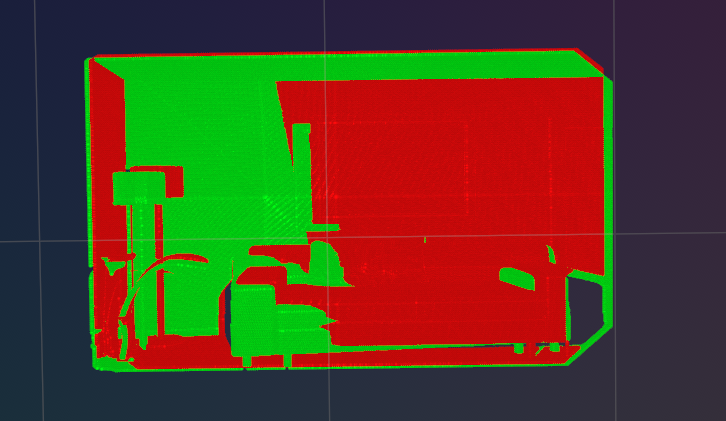
\includegraphics[width=0.45\textwidth]{2_3_f1.png}
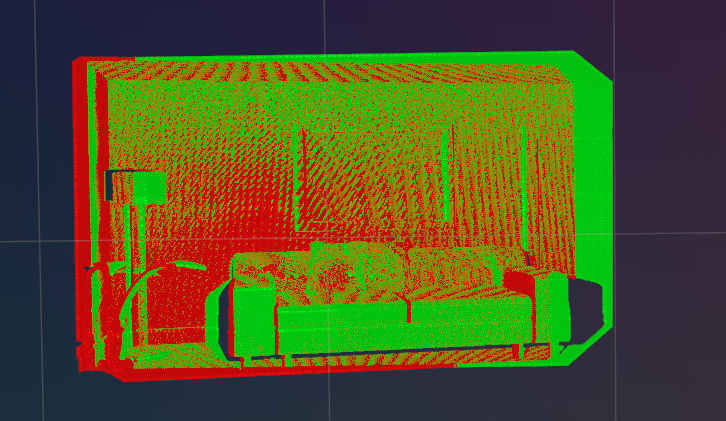
\includegraphics[width=0.45\textwidth]{2_3_f2.png}
\captionof{figure}{(a) Optimization between frames 10 and 50 after (a) 0 iterations (b) 10 iterations}
\end{center}


We clearly see that optimization between 10 and 100 fails. From the optimization logs, we see that the number of inliners starts at around 25k and slowly approachs 30k. This is in stark contrast to the optimization between frames 10 and 50, which starts with 70k inliers and reaches nearly 300k inliers near the end. This suggest that the shift between frames 10 and 100 lead to a large portion of pairs being initially filtered out due to the distance thresholding, and even though the loss metric between the existing paiirs is low, we simply don't have enough keypoints to fully match the scene.

\begin{center}
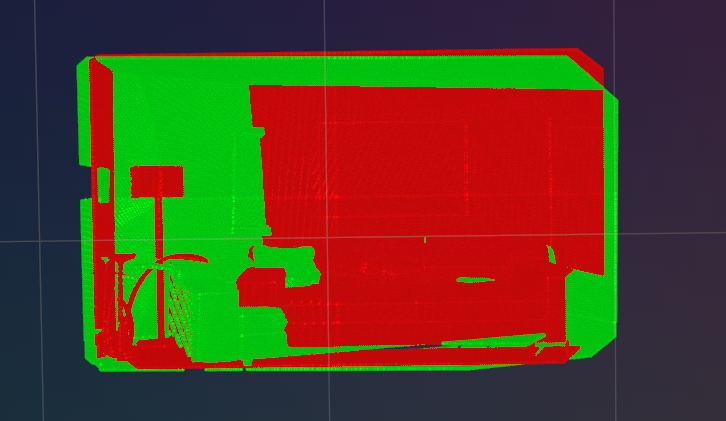
\includegraphics[width=0.45\textwidth]{2_3_f3.png}
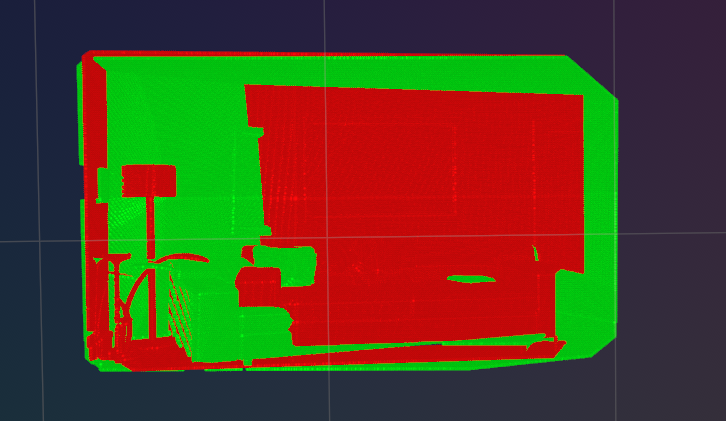
\includegraphics[width=0.45\textwidth]{2_3_f4.png}
\captionof{figure}{(a) Optimization between frames 10 and 100 after (a) 0 iterations (b) 10 iterations}
\end{center}

This problem is alleviated if we just capture enough keypoints. After 50 iterations, the number of matched pairs is around 225k and we see a much better matching.

\begin{center}
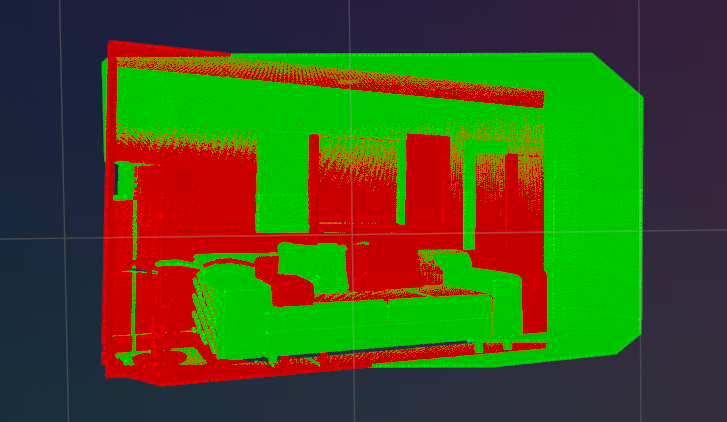
\includegraphics[width=0.45\textwidth]{2_3_f5.png}
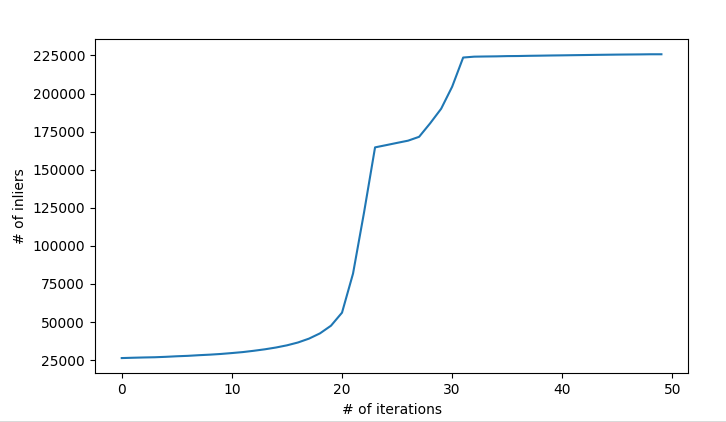
\includegraphics[width=0.45\textwidth]{2_3_f6.png}
\captionof{figure}{Optimization between frames 10 and 100 after 50 iterations (a) visualization (b) comparison of iteration number and \# of inliers}
\end{center}

\end{enumerate}

\section{Point-based Fusion}

\subsection{Filter}
Implementation in code

\subsection{Merge}

First convert the point $q$ from camera into world view, then combine with $p$ in a weighted manner. Don't forget to normalize:

\[ \frac{1}{w+1}(w \cdot p + R^w_cq + t^w_c) \]

We can do the same for the normals, though we need to do a different manner of normalization through dividing by the norm:

\[ \frac{1}{||w \cdot n_p + R^w_c n_q||} (w \cdot n_p + R^w_c n_q) \]

\subsection{Addition}
Implementation in code

\subsection{Results}
\begin{center}
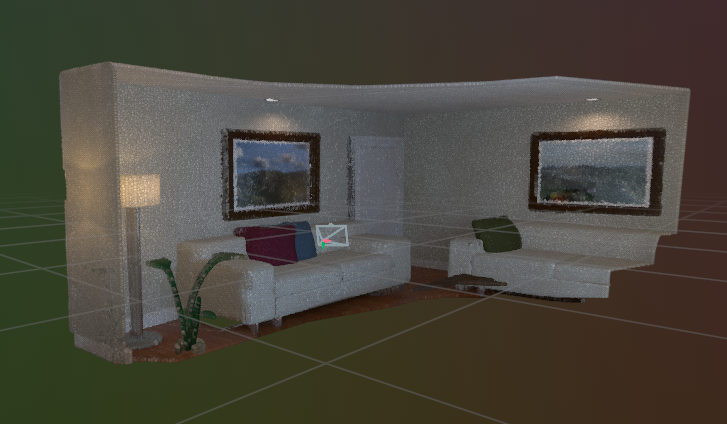
\includegraphics[width=0.45\textwidth]{3_4_f1.png}
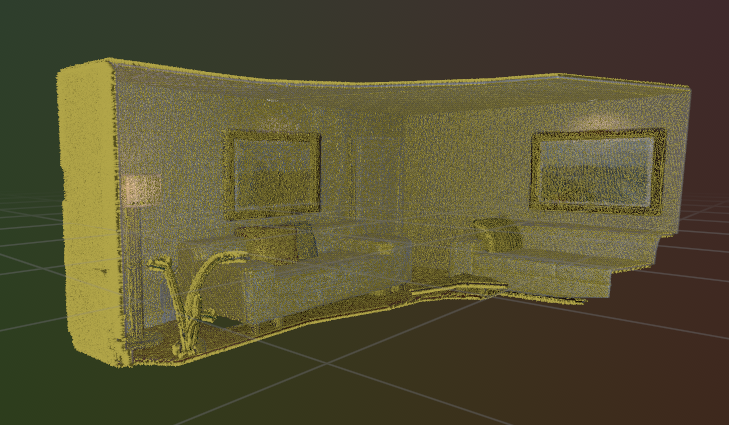
\includegraphics[width=0.45\textwidth]{3_4_f2.png}
\captionof{figure}{Visualization of fused images with a (a) rendered image (b) normal map}
\end{center}

At the end of the process, we had 3123765 points in total. Each RGB image has resolution 640 by 480 pixels; after downsampling, we should have 76800 pixels per image. For two hundred images, we'd have a total of 15360000 pixels, which implies a compression ratio of 80\% (i.e. we have compressed the number of points down to $100-80=20$\% of all points).

\section{The dense SLAM system}
\begin{enumerate}

\item  The input frame is the target and the map is the source. You cannot swap because the map has no image layout, i.e. no vertex map, to project into.

\item 

\begin{center}
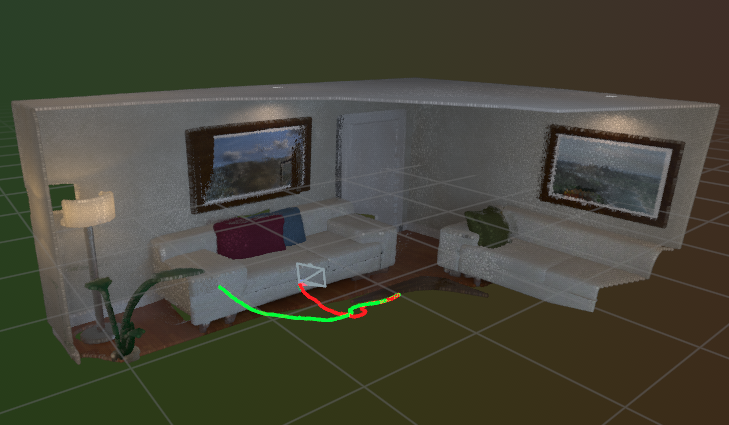
\includegraphics[width=0.8\textwidth]{4_f1.png}
    \captionof{figure}{Visualization of estimated (red) and true (green) trajectories}
\end{center}

Initially there is some deviation as the map is sparse and ICP has fewer correspondences. As more frames are fused, the map becomes denser and ICP converges more reliably, leading to the overlap between the estimation and ground truth that we observe. However, without loop closure, small errors accumulate over time, and drift would become more pronounced over longer sequences. However, in this specific scenario, this doesn't have any noticable effect due to the short length of the sequence.

\end{enumerate}

\end{document}
